\subsection{wiringPi}
Der NanoPi Neo2 Black kommt mit einem vorinstallierten Fork von der wiringPi Libarry
https://github.com/friendlyarm/WiringNP/blob/master/wiringPi/wiringPi.c
Die funktionalität der drei verwendetetn C-Funktionen werden im folgenden beschrieben.
\subsubsection{wiringPiI2CSetup}

Der Funktion wird beim audfruf die I2C Adresse übergeben mit welcher eine verbindung aufgebaut werden soll: wiringPiI2CSetup(address).\\
Der Rückgabewert ist der Standard Linux File Disciptor oder -1, falls ein Fehler auftritt. 
Die Anzahl der File Desciptoren ist begrenzt daher muss die verbindung mit der Funktion close() aus der Library: unistd.h geschlossen werden wenn sie nicht mehr benötigt wird.


\subsubsection{wiringPiI2CWriteReg8}
Der Funktion wird bei aufruf der File Desciptor einer I2C verbindung sowie ein ziel register und die zu schreibenden 8bit Daten übergeben: wiringPiI2CWriteReg8 (fd, RegAdr, 8-Bit-Data).
Wenn der Schreibzugriff vom I2C gerät bestätigt wurde wird eine 0 zurück gegeben.
\subsubsection{wiringPiI2CReadReg8}
Der Funktion wird bei aufruf der File Desciptor einer I2C verbindung sowie ein ziel register übergeben: wiringPiI2CReadReg8(fd, RegAdr).
Der ausgelsene 8-Bit inhalt des Register ist der rüchgabewert.
Wenn das Lesen Fehlschlägt bleibt das Programm in einer Endlosschleife hängen.

\subsection{AS726X Libary}
Die WiringPi\_AS726X\_Libary enthält alle funktionen um den AS7261 und AS7265X zu steuern und auszulesen.
Da die Beispielimplementierungen im Datenblatt in vielen detaifragen ungenau und Fehlerhaft ist wurde die Arduino OpenSource Libarrys von sparkfun SparkFun\_AS726X\_Arduino\_Library-master und SparkFun\_AS7265x\_Arduino\_Library als implementierungs grundlage verwendet.
Im ersten schritt der entwirklung wurde sie für die I2C schnittschelle WiringPi des NanoPi umgeschrieben und anschließen in ihrer Funktionalität erweitert um für das messystem mit mehreren sensoren auf dem gleichen bus nutzbar zu sein. \\

Im Folgenden Text werden die Register Adressen und mit den gleichen Namen wie im source code bezeichnet die Numerische Adressen sind in Tabelle \ref{TODO} aufgelistet. TODO table

\begin{figure}[H]
\centering
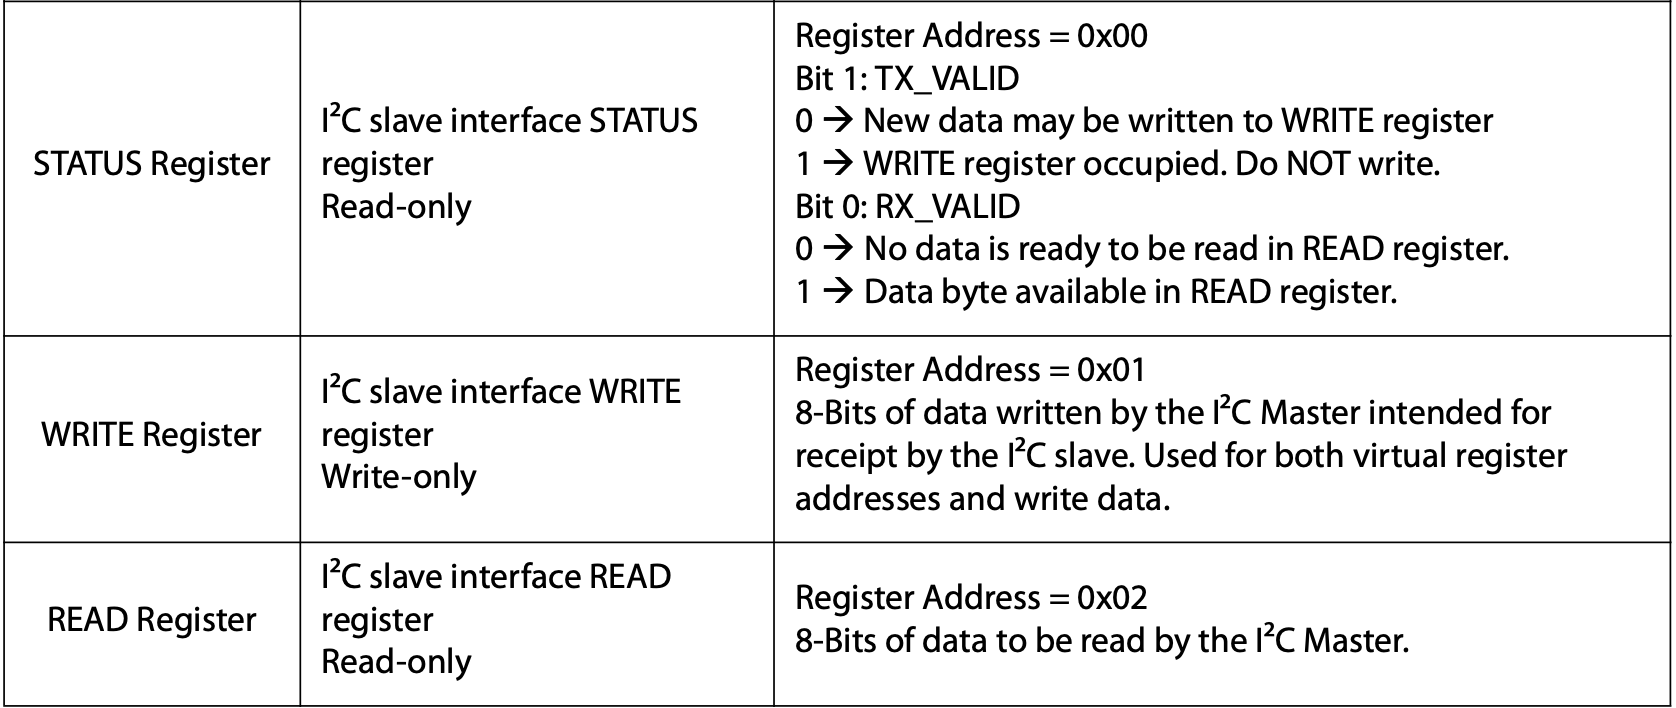
\includegraphics[width=0.75\textwidth]{img/PysicalRegister}
%\caption*{Quelle: Datenblatt AS7261}
\caption{PysicalRegister}
\label{fig:Seitenasicht-AS726X}
\end{figure}

\begin{figure}[H]
\centering
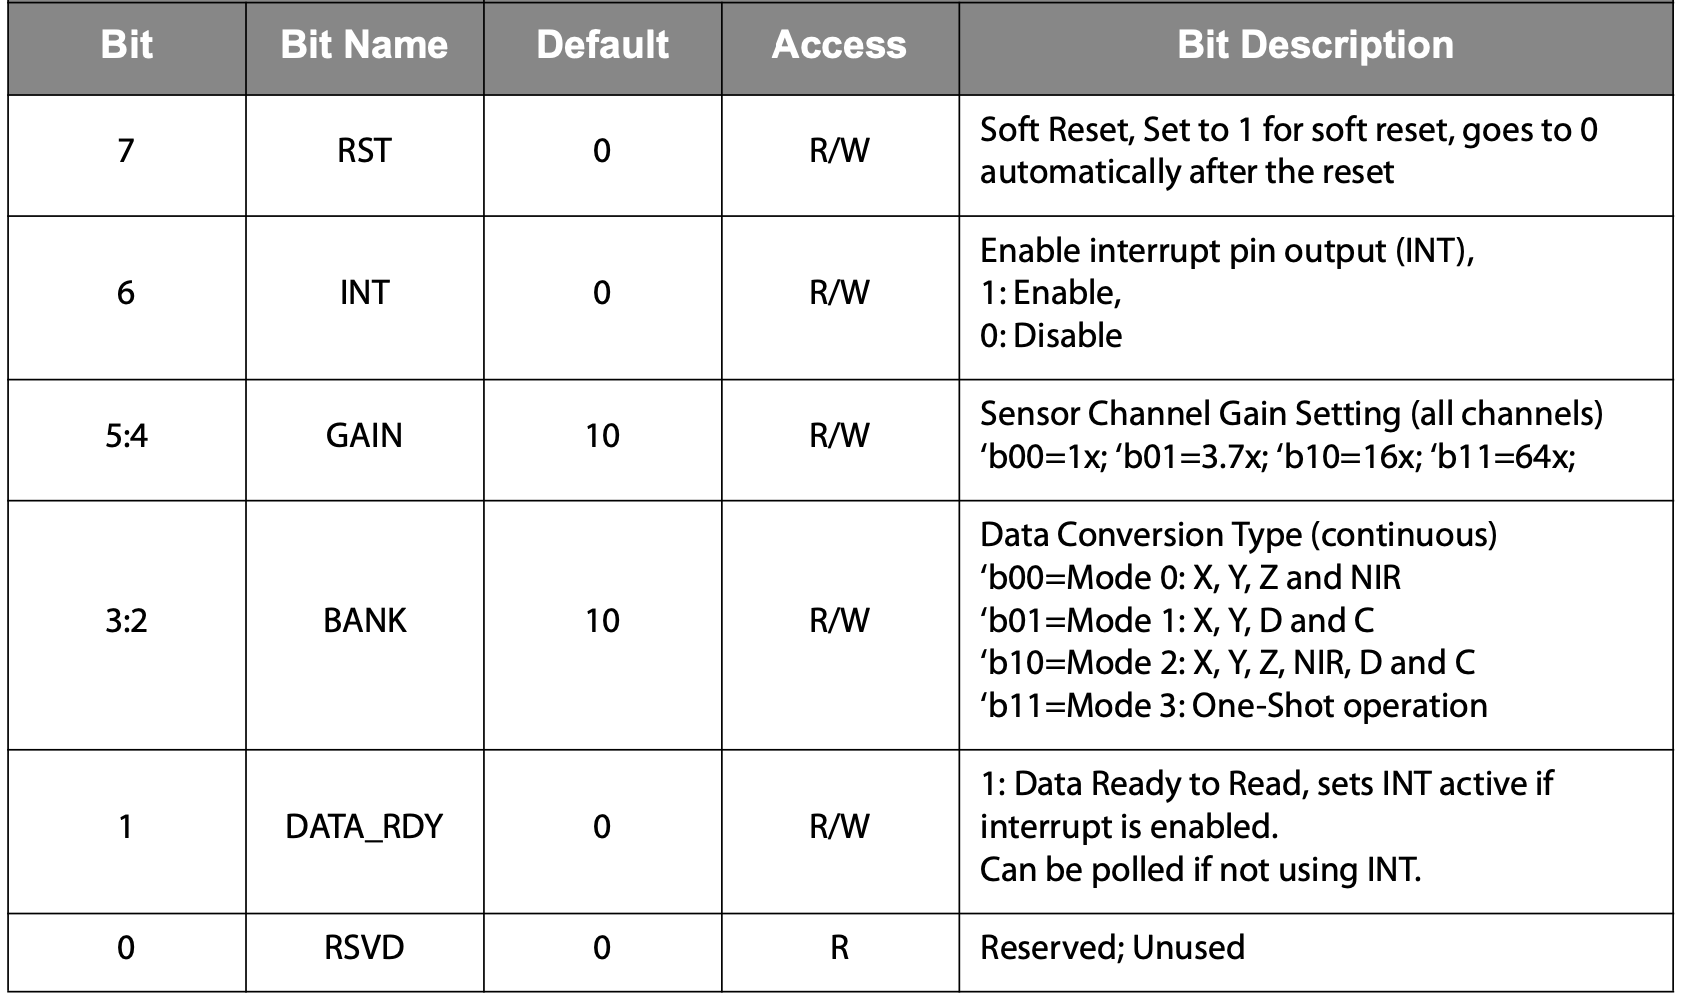
\includegraphics[width=0.75\textwidth]{img/ControlRegister_2}
%\caption*{Quelle: Datenblatt AS7261}
\caption{AS726x\_CONTROL\_SETUP}
\label{fig:Seitenasicht-AS726X}
\end{figure}

\subsubsection{virtualWriteRegister}
Wie bei Embeddet geräten üblich werden Einstellungen auf dem sensor verändern indem verschiedene sogenannte Special function registers  mit daten beschrieben werden.\\
Jedes Special function register ist 8Bit groß und hat eine adresse und
jedes Bit des Register representiert eine einstellung.
Beispielsweise ist 0x07 das LED Control Register des Sensors.
Bit 0 des Registers Beschreibt den Zustand der Status LED.
Die Restlichen 7 Bit des Registers Beschreibt den Zustand anderer LEDs die für den Messaufbau aber irrelevant sind.\\
Wird register 7 mit dem Dezimal wert 0 beschrieben sind alle LED aus, wird es mit dem Dezimal wert 1 beschrieben leuchtet ist nur die status LED.
Die Register Lassen sich aber nicht direkt Beschreiben, stattdesswen sind sie als sogennate Virtuelle Register Implementiert.

Der Sensor arbeitet mit virtuellenRegistern.
Das heißt das nur Register 0x01 (WRITE Register) beschrieben werden kann.
Um daten in eins der Special Funktions Register zu schreiben wird die funktion virtualWriteRegister verwendet.
Die Funtionsweise lässt sich in 4 schritten zusammnefassen:
\begin{itemize}
	\item Zeile TODO Warten bis das WRITE Register leer ist, was angezeigt wird indem  das Bit AS72XX\_TX\_VALID im  Register AS72XX\_STATUS\_REG den wert 1 annimmt.
	\item Zeile TODO Schreibe die Virtuelle Adresse in das WRITE Register und Setze zusätzlich Bit 8 des WRITE Register auf 1 um zu zeigen das es sich um einen Schreibenden zugriff auf das Virtuelle Register handelt.
	\item Warte erneut bis das WRITE Register leer ist.
	\item Schreibe die Daten in das WRITE Register
\end{itemize}
Der Sensor wird jetzt selber die übertragenen Daten aus dem WRITE Register angebene Virtuelle Register kopieren.
\lstinputlisting[language=C,style=c]{code/virtualWriteRegister.c}
\subsubsection{virtualReadRegister}
Die Unterschiedlichen Messdaten des Sensors werden in dedizierten registern gespeichert.
 Es ist aber nur über den indirekten weg des AS72XX\_READ\_REG und der Virtuellen Register Adressen möglich daten auszulesen.
Die Funktionsweise der zum Daten auslesen benötigten funktion virtualReadRegister lässt sich wieder in 4 schritte aufteilen.
\begin{itemize}
	\item Das AS72XX\_READ\_REG wird ausgelesen ohne das die daten verabeitet werden. Dieser schritt ist wie ein Reset des Registers zu verstehen.
	\item Zeile TODO Schreibe die Virtuelle Adresse in das WRITE Register und Setze zusätzlich Bit 8 des WRITE Register auf 0 um zu zeigen das es sich um einen Lesenden zugriff auf das Virtuelle Register handelt.
	\item Sobald das AS72XX\_STATUS\_REG den wert AS72XX\_TX\_VALID annimmt sind die Daten aus dem angebenen Virtuellen Register in das AS72XX\_READ\_REG kopiert worden.
	\item Lese die Daten aus dem S72XX\_READ\_REG
\end{itemize}
\lstinputlisting[language=C,style=c]{code/virtualReadRegister.c}

\subsubsection{MeasurementFromAdress}
Die Funktion baut einen I2C Verbindung zur übergebenen Bus-Adresse auf und  ruft die Funktion takeMeasurments mit dem File Descriptor der aktiven I2C Verbindung auf.
Nachdem die Funktion takeMeasurements durchlaufen ist wird die I2C Verbindung wieder geschlossen.
\lstinputlisting[language=C,style=c]{code/MeasurementFromAdress.c}

\subsubsection{takeMeasurements}

Die Funktion takeMeasurements ruft die Funktion setMeasurementMode mit dem Parameter 3 auf das setzt den aus \ref{todo} bekannten Bankmode der übergebenen I2C Verbindung (fd) auf Bank Mode 3.
	Die On-Shot Messung wird sofort gestartet, in Zeile 9 wird gewartet bis die Messung abgeschlossen ist. 
		Um sicherzustellen das die funktion DataAvailable richtig arbeitet muss vor der Messung das Flag DataAvailable auf 0 gesetzt werden (Zeile 3).
Die Daten werden hier nicht ausgelesen daher gibt es keinen rückgabewert.\\
\lstinputlisting[language=C,style=c]{code/takeMeasurements.c}

\subsubsection{setMeasurementMode}
Mit der Funktion setMeasurementMode werden die Bankmode Bits 2 und 3 des AS726x\_CONTROL\_SETUP Registers mit dem gewünschten wert für den Bankmode beschrieben.\\
Da die anderen Bits des Registers noch weitere einstellungen repräsentieren welche nicht verändert werden sollen, muss das register erst ausgelsen werden.
Anschließend werden die Bankmode Bits auf 0 gesetzt um im nächsten schritt mit dem gewünschten neuen Bankmode wert beschrieben zu werden. 
Die Bedeutung der Bankmodes ist in \ref{TODO} erleutert.
\lstinputlisting[language=C,style=c]{code/setMeasurementMode.c}
\subsubsection{dataAvailable \& clearDataAvailable}
Das Bit dataAvailble im register todo wird vom Sensor auf 1 gesetzt wenn nach einer Messung neue daten vorhanden sind, Intterupts müssen dafür ausgeschaltet sein.
dataAvailble wird auf 0 gesetzt wenn daten gelsen werden.
Wenn eine One-Shot messung im Bankmode 3 durchgeführt wird sollte das dataAvailble bit mit der Funktion clearDataAvailable auf 0 gesetzt werden, da nicht sicher gestellt ist das die daten vor der Messung gelsen wurden. Es besteht die möglichkeit das sich das bit fälschicherweise noch im falsch positiven zustand befindet.
Die Funktion dataAvailable gibt den wert des DataAvailable Bit zurück.
\lstinputlisting[language=C,style=c]{code/dataAvailable.c}
\subsubsection{Rohwerte des AS7261 Auslesen}
Die in \ref{todo} beschrieben 6 Channel des AS7261 werden mit den folgenden Funktionen ausgelesen:
\begin{itemize}
	\item getX\_CIE(fd)
	\item getY\_CIE(fd)
	\item getZ\_CIE(fd)
	\item getNIR(fd)
	\item getDark(fd) 
	\item getClear(fd)
\end{itemize}
Der File Deskriptor einer I2C Verbindung mit einem AS7261 und das zu lesende Register wird als Übergabe Parameter erwatet.\\
Um den Messwert auszulesen, wir die Funktion getchannel aufgerufen.
Der Rückgabewert ist der 16-Bit Messwert aus dem jeweiligen Register vom Datentyp integer.

\subsubsection{getChannel}
Da die Messdaten 16-Bit groß sind, der Sensor aber nur über 8 Bit register verfügt werden 2 aufeinader folgende register ausgelsen und im Big-Andian Format aneinader geheftet.
Die Funktion getChannel erwatet den File Disciptor einer I2C verbindung zu einem Sensor und die adressen des High Bytes eines Raw Data Registers.
Der Rückgabewer ist der 16-Bit Messwert aus dem jewaligen Register vom Datentyp Integer.
\subsubsection{Rohwerte des AS7265X Auslesen}
Da der bei daten lesen des AS7265X 3 sensoren unter der gleichen adresse erreichbar sind muss zusätzlich zum File Disciptor und des ziel Registers der Device Identifier angeben werden.
Folgende Rohdaten können ausgelsen werden:
\begin{center}
\begin{tabular}{ c c c }
 	AS72651 & AS72652 & AS72653 \\ 
 	getR & getG & getA \\  
 	getS & getX & getB \\
 	getT & getI & getC \\  
 	getU & getJ & getD \\
 	getV & getK & getE \\  
 	getW & getL & getF \\
\end{tabular}
\end{center}
Um den Messwert auszulesen, wir die Funktion getChannel\_AS7265X aufgerufen.\\
Der Rückgabewert ist der 16-Bit Messwert aus dem jeweiligen Register vom Datentyp integer.

\subsubsection{getChannel\_AS7265X}
Die Funktion verarbeitet den aus \ref{Rohwerte des AS7265X Auslesen} bekannten Device Identifier indem die Funktion selectDevice aufgerufen wird.
	Da es aber keine möglichktet gibt zu überprüfen ob der gerätewechsel erfogreich war muss voher überfrüft werden ob das jewalige slave gerät AS72652 oder AS72653 vorhanden ist.
	Ist ein Slave nicht vorhanden wird der wert -1 zurück gegeben.
	Ohne dieses überprüfung werden wert aus den gleich numerierten registern des AS72651 ausgelsen obwohl werte eines nicht vohrandnen oder falsch aufgelöteten slave sensors erwatet werden.
	Das eigentlich auslesen des 16-Bit Messwerts erfolgt mithilfe der Funktion getChannel, das ergebnis ist rügbaewert der Funktion getChannel\_AS7265X.

\subsubsection{selectDevice}
Die Notwendigkeit für selectDevice wurde in ref{getChannel\_AS7265X} bereits erleutert.
Laut Datenblatt sollen nur die Bits 0 und 1 des DEV\_SELECT\_CONTROL registers beschrieben werden, das stimmt aber nicht.\\
In der Realität muss das gesamte 8-bit register mit folgenden werten beschriebn werden um beim aschnliesenden lesen vorgang  daten vom jewaligen sensor zu erhalten.
\begin{center}
\begin{tabular}{ c c }
 	DEV\_SELECT\_CONTROL & Sensor \\ 
 	0x00 & AS72651 \\  
 	0x01 & AS72652 \\
 	0x02 & AS72653 \\  
\end{tabular}
\end{center}

\subsubsection{Kalibrierte Werte des AS7261 Auslesen}
TODO
\subsubsection{Kalibrierte Werte des AS7265X Auslesen}
TODO
\subsubsection{getCalibratedValue}
TODO
\subsubsection{convertBytesToFloat}
\subsubsection{Enable/Disable Indicator}
Mit der Funktion enableIndicator wird das 0 Bit des AS726x\_LED\_CONTROL Register aus 1 gesetzt, so wird die Rote status led des jewaligen sensors auf dem sensorbaord angeschaltet.\\
Mit der Funktion dnableIndicator wird das gleiche Bit auf 0 gesetzt, also die Led ausgeschaltet.\\
Als übergabe paramter wird bei beiden funktionen der FileDiskiptor einer aktiven I2C verbindung erwatet.\\

\subsubsection{softReset}
Der Sensor liefert in einigen situationen messwerte auserhalb des erwatungsbereiches.
Dieses Problem kann in manchen fällen behoben werden indem ein softReset durchgeführt wird.
Da in der hier beschrieben Implenatation keine Fehler aufteten wie die funktion nicht benötigkt, kann aber in zukünftigen versionen verwendet werden.

Die Funktion softReset setzt das 8 Bit des Registers CONTROL\_SETUP auf 1 um einen softReset auszulösen.
Der datenbaltt gibt an das mindestens 1000ms gewatet werden muss bevor der softReset abgeschlossen ist und der sensor wieder genutzt werden kann.
Als übergabe paramter wird bei beiden funktionen der FileDiskiptor einer aktiven I2C verbindung erwatet.
\subsubsection{I2CScan}
Die Funktion I2CScan wird zu begin des Programms aufgerufen um zu erfassen welche Sensoren mit dem I2C DatenBus verbunden sind.
Die die gefunden Sensor Adressen und der Sensortyp werden in das struct sensor\_list geschrieben.\\
Außerdem werden die im Terminal ausgegeben damit der Benutzer überprüfen kann ob alle erwatetn sensoren erkannt werden.\\
Als Übergae paramter wird im call by refrence style ein Pointer zu einem Struct vom typ sensor\_list erwatet.
Da die daten direkt in das extern deklarierte(?) strukt geschriebn wird gibt es keinen rückgabe wert.
Um die angeschlossenen sensoren zu detetieren wir zu jeder der $2^8$ möglichen I2C adressen eine verbindung aufgebaut und schreibversuch mithilfe der funktion wiringPiI2CWriteReg8 vorgenommen.
Wenn die Funktioon wiringPiI2CWriteReg8 eine 0 zurück gibt war der Schreibversuch erfogreich also muss ein sensor unter dieser adresse vorhanden sein.
Das im datenblatt nicht erwähnte register mit der adresse 0x05 wurde ausgewählt das es mit dem wert 0x01 beschriebn werden kann ohne das der sensor sein verhalten verändert.
Die funktion getVersion wird genutzt um die version des gefunden sensors zu ermitteln.
Wenn ein AS72651 erkannt wird wird zusäzlich abgefragt ob auch die slave sensoren AS72652 und AS72653 vorhanden sind, diese information wird nur im Terminal ausgegebn und nicht is das struct sensor\_list geschrieben, da es für den programmablauf nicht notwendig ist.
\subsubsection{getVersion}
Die funktion getVersion gibt den inhalt der Registers AS726x\_HW\_VERSION zurück, indem der zurückgebene wert mit den beiden SENSORTYPE werten verglichen wird(SENSORTYPE\_AS7261 und SENSORTYPE\_AS72651). kann festegellt werden um welchen sensor es sich handelt. 
Als übergabe paramter wird bei beiden funktionen der FileDiskiptor einer aktiven I2C verbindung erwatet.\\

\subsubsection{scanAS7262}
Als übergabe paramter wird bei der funktionen der FileDiskiptor einer aktiven I2C verbindung mit einem AS72651 erwatet.\\
Die funktion überprüft den status des 4. Bit des registers DEV\_SELECT\_CONTROL und gibt ihn zurück. Das Bit ist auf 1 gesetzt wenn der slave sensor AS7262 vorhanden ist, im falle der abwesenheit ist es 0.\\
Im Datenbaltt des AS7265X wird fälschicherweise angegeben das das 5. Bit überprüft werden muss.

\subsubsection{scanAS7263}
Als übergabe paramter wird bei der funktionen der FileDiskiptor einer aktiven I2C verbindung mit einem AS72651 erwatet.\\
Die funktion überprüft den status des 5. Bit des registers DEV\_SELECT\_CONTROL und gibt ihn zurück. Das Bit ist auf 1 gesetzt wenn der slave sensor AS7262 vorhanden ist, im falle der abwesenheit ist es 0.
\subsubsection{setGain}
Die Messergebnisse der Sensoren können intern verstärkt werden, das ist beispielsweise in dunklen messumgebenungen oder bei gebrauch von relativ licht undurchlässigen streuscheiben notwendig.\\
Um den Verstärkungsfaktor einzustellen wird die Funktion setGain benötigt.\\
Die Funktion setGain beschreibt das 4 und 5 Bit des registers CONTROL\_SETUP mit einem der 4 möglichen zustände welcher an die Funktion sie übergebenen wird.

\begin{tabular}{ l l}
 	Wert & Verstärkungsfaktor \\ 
 	0 & 1x (power-on default) \\  
 	1 & 3.7x \\
 	2 & 16x \\  
 	3 & 64x \\
\end{tabular}


Ist der übergebe wert größer als 3 ist wird das register auf den Wert 3 gesetzt.
\subsubsection{setIntegrationTime}
Um die integrationszeit der Messung einzustellen wird in das register AS726x\_INT\_T ein wert (integrationValue) zwischen 0 und 255 geschrieben, die Integrationszeit errechnet sich indem dieses wert mit dem Faktor 2.8ms multipliziert wird.
Die funktion setIntegrationTime erwatet als übergabeparamter das integrationValue sowie den FileDiskiptor einer aktiven I2C verbindung.\\

\subsubsection{disableInterrupt}
Die Funktion disableInterrupt setzt das INT Bit im register AS726x\_CONTROL\_SETUP auf 0 um Interrupts aus zu schalten.
Da Der Interrupt auf der Sensor Paltiene nicht verbinden ist muss .. toto muss dass wirklich?

\subsection{influxDB Library writeToDatabase}
Um die Messdaten der Sensoren in die aus \ref{datenbankundinterface} bekannte InfluDB zu schreiben wurde die influxDB Library entwikelt, sie enhält nur eine einzige nach außen sichtbare funktion: writeToDatabase.
\subsubsection{writeToDatabase}
Um die Datenbenk zu beschreiben muss zuerst ein Socket geöffnet werden um mit der influxdb server instanz zu verbinden.
der UnfluxDB sever ist unter der locallink adresse 127.0.0.1 am port 8086 zu erreichen.
	Diese Werte können in der influxdb.h datei angepasst werden falls in zukunft die notwendigkeit besteht den server auf einem externen gerät zu betreiben.\\
	Die Komunikation mit dem Influxdb server erflogt über das Http basierte InfluxDB line protocol.

	
	In zeile 68 wird der Datenbankname , Username,  Passowrt der Datenbank und die größe des Body's der anfage in den header teil der http anfrage geschrieben.
	
	In zeile 64 wird der body teil der anfrage im InfluxDB line protocol format erzeugt, dieser enthält den Bezeiner des Messwerts (z.B. A oder B), die I2C adresse des jewaligens Sensors von dem die Messdaten stammen, den Messert selbst sowie den Zeitstempel der Messung in ms.
	
In zeile 85 wird der Http request bestehend aus Header und Body an den Server übertragen.
Die antwort vom Server wird gespeichert und anschließen auf die erwatete rückmeldung "HTTP/1.1 204 No Content" untersucht, wenn der schreibversuch fehlschlägt wird eine meldung im Terminal angezeigt(TODO hier sollte die status led sich verändern).
\subsection{main}
In der Mainfunktion kommen 



